\chapter{Revisão Bibliográfica}
	\chapterprecis{Teste, teste}
	
	\section{Laboratório de Operações e Processos - Contextualização}
		O Laboratório de Operações e Processos (LOP) é um dos diversos laboratórios para fins de ensino e pesquisa pertencentes ao Departamento de Engenharia Química da UFMG (DEQ). Ainda existem outros laboratórios vinculados ao departamento cuja finalidade é prestar serviços às comunidades interna e externa à UFMG \footnote{\url{http://www.deq.ufmg.br/departamento/infraestrutura}}.
		
		O LOP possui quatro plantas didáticas: \textbf{explicar aqui brevemente as 4 plantas constituintes do laboratório}
		
		%explicar aqui agora sobre a planta de trocador existente
		O trocador de calor existente no laboratório, cuja imagem pode ser vista na \autoref{fig:lab}, é do tipo tubular. Este sistema, que é fabricado e fornecido pela Universidade de Santa Cecília\footnote{\url{http://cursos.unisanta.br/quimica/laborato/index.html}}, foi adquirido pela UFMG em 2002\footnote{Item 35 do catálogo disponível em: \url{http://cursos.unisanta.br/quimica/laborato/LOU-2016.pdf}}. Originalmente, a planta possui um botão para ligar e desligar bomba e aquecedor simultaneamente, bem como conta com 4 sensores de temperatura, cujos valores são exibidos e display LCDs. A medição de vazão de água quente era inferida através da utilização de uma Calha Parshall\footnote{Funcionamento da Calha Parshall: \url{http://www.dec.ufcg.edu.br/saneamento/PARSHALL.html}}, e a medição de água fria, através da indicação de um rotâmetro\footnote{\url{http://www.sensorsmag.com/components/basics-rotameters}}
		
		\begin{figure}[!htb]
			\centering
			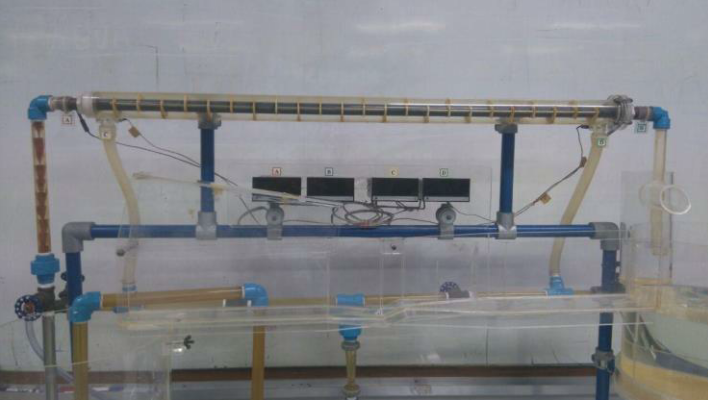
\includegraphics[scale=0.7]{lab}  %pode alterar o tamanho
			\caption{Trocador de Calor presente no LOP.}
			\label{fig:lab}
		\end{figure}

			
		Em 2016, um projeto de modernização desta planta foi iniciado por \cite{luiz2016}.  O projeto consistiu na implementação de um sistema embarcado para operação local e controle da planta. Para alcançar o objetivo, foram feitos os seguintes passos:
		\begin{itemize}
			\item 
			Instalação de quatro novos sensores de temperatura, dois novos sensores de vazão, tornando possível a medição digital das vazões; 2 relés, para o controle do acionamento dos atuadores e um inversor de frequência para controlar a rotação da bomba;
			\item 
			Instalação de um Arduino Due \footnote{\url{https://store.arduino.cc/usa/arduino-due}} para fazer a interface com sensores e atuadores, processar os algoritmos de controle, e exibir os dados em um display LCD. O programa criado no Arduino possibilita a operação em modo automático e manual;
			\item 
			Construção e instalação de um painel para operar e visualizar os dados da planta. Através desse painel é possível selecionar o modo de funcionamento da planta (manual ou automático). Em modo manual, é possível ligar e desligar bomba e aquecedor, bem como controlar a velocidade da bomba e potência do aquecedor. O display LCD permite exibir várias informações como por exemplo valores das temperaturas e vazões, bem como a sintonia dos controladores. Essas informações não conseguem ser expostas ao mesmo tempo para o usuário, portanto um sistema de navegação foi implementado no Arduino. O esboço do painel elaborado é mostrado na \autoref{fig:painel}.
		\end{itemize}
			
			\begin{figure}[!htb]	
				%\centering
				\captionsetup{justification=centering}
				\begin{center}
					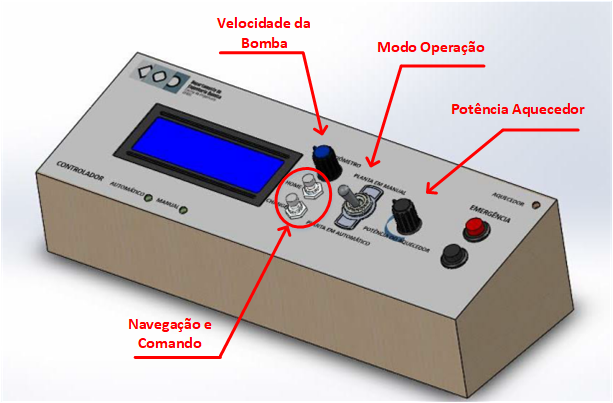
\includegraphics[scale=0.6]{painel}  %pode alterar o tamanho
					\caption[Painel instalado na planta de trocador de calor]{\label{fig:painel}Painel instalado na planta de trocador de calor. \\Adaptado de \cite{luiz2016}}
				\end{center}		
			\end{figure}
		
			A Arquitetura do sistema finalizado é exibida na \autoref{fig:arq_atual}. Destaca-se o fato que não foi possível integrar o controle da potência do aquecedor no Arduino, sendo enviado diretamente do painel. Apesar de previsto no projeto, nenhum algoritmo para controle em malha fechada foi programado.
		
			\begin{figure}[!htb]	
				%\centering
				\captionsetup{justification=centering}
				\begin{center}
					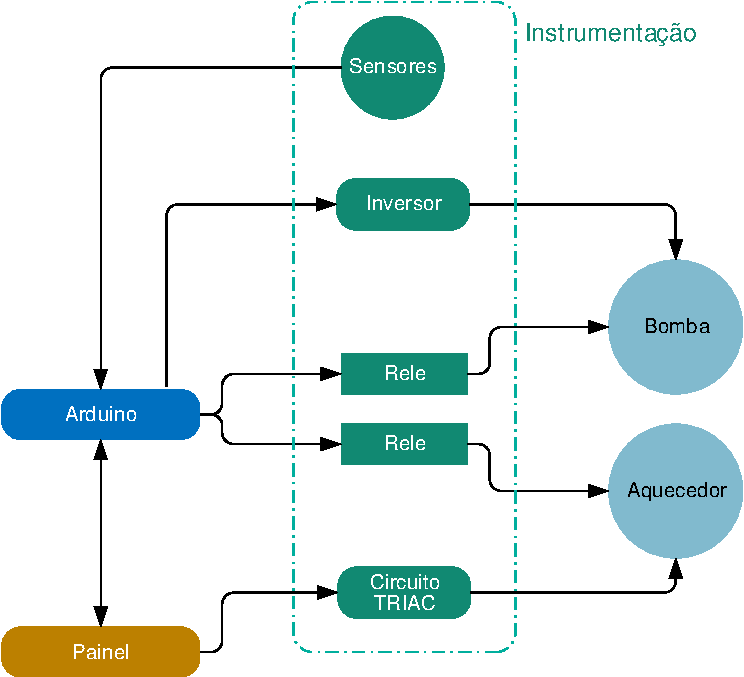
\includegraphics[scale=0.8]{arq_atual}  %pode alterar o tamanho
					\caption[Arquitetura do sistema instalado]{\label{fig:arq_atual}Arquitetura do sistema instalado}
				\end{center}		
			\end{figure}
		
	
	\section{Tecnologias para Controle e Monitoramento de Processos}
		\label{sec:rev_monitor}
		A seguir são apresentadas algumas tecnologias utilizadas para implementar sistemas de controle e monitoramento de processos.
		
		\subsection{Sistemas SCADA}
		Aplicações SCADA são utilizadas na supervisão e controle de largamente empregadas na indústria em setores como saneamento, energia, metalurgia, manufatura entre outros \cite{pablo2011}. Estes sistemas coletam dados de dispositivos de campo e os concentram em ambientes onde possam ser processados e armazenados. Os operadores podem visualizar esses dados através de interfaces gráficas (IHMs), que ilustram o que está ocorrendo na planta em tempo real. 
		
		A arquitetura de um sistema SCADA é mostrada na \autoref{fig:pc_plc}. Estes sistemas são compostos por componentes que são definidos na literatura de acordo com a contribuição no processo de coleta, processamento e exibição dos dados de uma planta.
		
		\begin{figure}[!htb]	
			%\centering
			\captionsetup{justification=centering}
			\begin{center}
				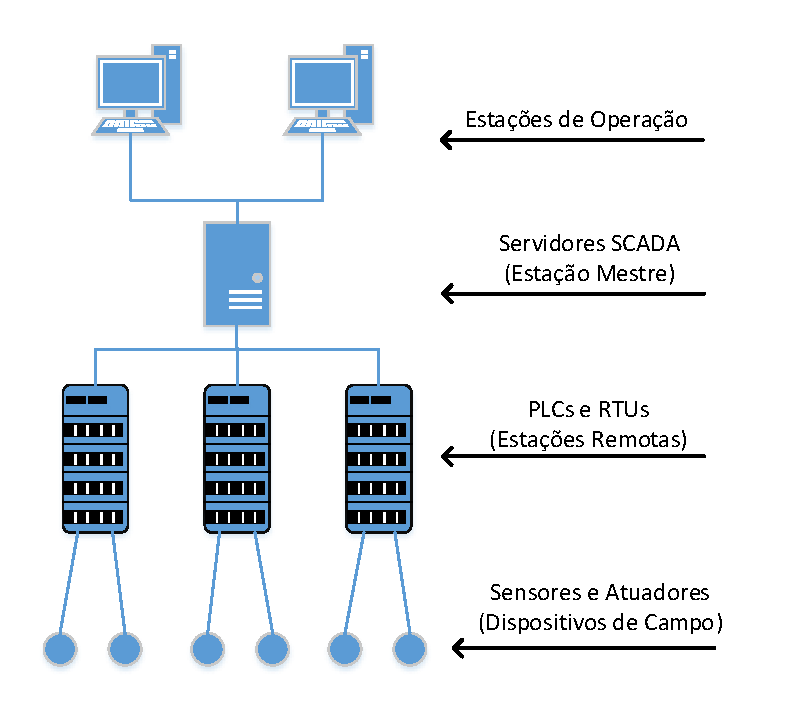
\includegraphics[scale=0.5]{pc_plc}  %pode alterar o tamanho
				\caption[Arquitetura do sistema instalado]{\label{fig:pc_plc}Arquitetura do sistema instalado. Adaptado de \textcite{pablo2011}}
			\end{center}		
		\end{figure}
	
		Dispositivos de campos podem ser entendidos pelos sensores e atuadores. Os sensores medem grandezas físicas do processo. enquanto os atuadores interferem no processo como por exemplo através  acionamento de bombas e válvulas. 
	
		As estações remotas são dispositivos programáveis que possuem a função de fazer a interface entre dispositivos de campo e estações mestre, além de serem dotados de capacidade de executar algoritmos de controle local. Nessa categoria enquadram-se os CLPs e RTUs. Os CLPs surgiram no contexto de chão de fábrica, ou seja, necessidade de programação e menor alcance de comunicação, devida a pequena distância entre os equipamentos. As RTUs surgiram da necessidade de enviar dados de sistemas localizados a grandes distâncias da estação mestre. Contudo, a evolução desses equipamentos tornou difícil a distinção entre eles \cite{bailey2003}.
		
		As estações mestres são o cérebro do sistema. Elas são responsáveis por solicitar dados das estações remotas, processá-los, armazená-los, bem como repassar comandos dos operadores para as estações remotas. As estações mestres são computadores, cuja capacidade depende do porte do projeto. Existem diferentes fabricantes de software que podem ser executados nesses servidores. Alguns fabricantes disponibilizam a opção de separar o processamento em diferentes estações mestres.
		
		As estações de operação executam um software que apresenta uma interface gráfica para o usuário, em que o operador consegue visualizar e interferir no processo através de controles (botões, sliders, etc) disponibilizados pela interface. Em pequenas aplicações, as estações de operação e as estações mestres se encontram nos mesmos computadores.
	
		A comunicação entre estação mestre e remota se dá pela utilização de protocolos industriais abertos como por exemplo Modbus\footnote{\url{http://www.modbus.org/}}, DNP3\footnote{\url{https://www.dnp.org/Default.aspx}}, OPC\footnote{\url{https://opcfoundation.org/about/what-is-opc/}}, entre outros; também há a comunicação através de protocolos proprietários. Este último caso ocorre em sua maioria quando a estação mestre e remota são fornecidos pelo mesmo fabricante.
	
	\subsection{Tecnologia Embarcada}
		Como mencionado no \autoref{cap:introducao}, os sistemas embarcados, estão cada vez mais presentes no setor industrial. \textcite{yu2011}, fazem uma pesquisa sobre os modelos de sistemas embarcados e em quais tipos de aplicações industriais estão sendo utilizados.
		
		Destacam-se a utilização de microcontroladores para executar algoritmos de controle e comunicação com outros sistemas. Um estudo de caso cita o túnel de vento instalado na Universidade de Bradley. A arquitetura do sistema implantado é mostrada na \autoref{fig:lab_view}. Comparando com a arquiteura SCADA descrita anteriormente, os elementos marcados com o número 1, seriam os dispositivos de campo, o microcontrolador (2), seria a estação remota, o PC executando o LabView (3) seria a estação master, e o outro computador seria a estação de visualização (IHM).
		
		\begin{figure}[!htb]	
			%\centering
			\captionsetup{justification=centering}
			\begin{center}
				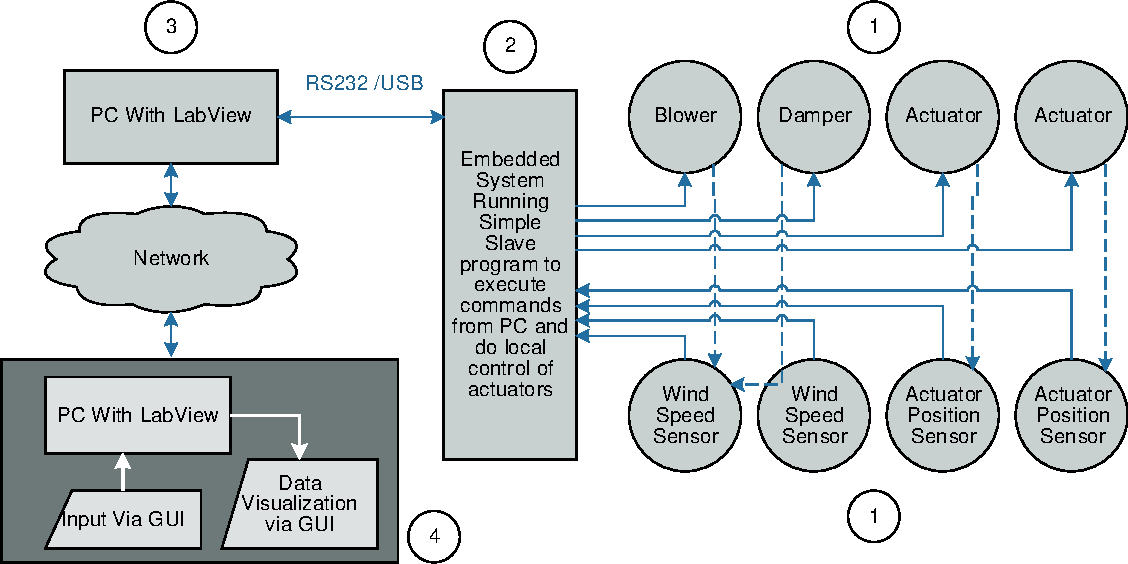
\includegraphics[width=15cm]{lab_view}  %pode alterar o tamanho
				\caption[Exemplo de Sistema com tecnologia embarcada]{\label{fig:lab_view}Exemplo de Sistema com tecnologia embarcada. Adaptado de \textcite{yu2011}}
			\end{center}		
		\end{figure}
	
		O estudo ainda menciona sobre crescimento na utilização de FPGAs, devido a redução dos custos de produção \duvida{continuar}
	